\chapter{Literature Review}\label{ch:literature}

\section{Introduction}\label{sec:intro}


\begin{figure}[H]
	\begin{subfigure}[b]{0.4\textwidth}
		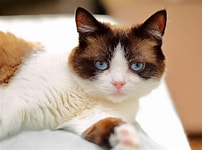
\includegraphics[width=\textwidth]{files/imgs/cat.jpg}
		\caption{Picture 1}
		\label{cat1}
	\end{subfigure}

	\begin{subfigure}[b]{0.4\textwidth}
		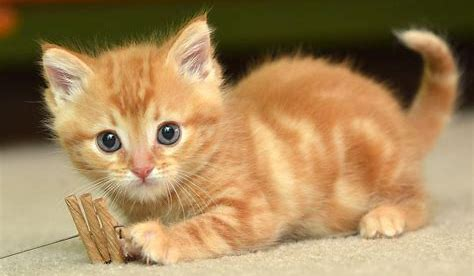
\includegraphics[width=\textwidth]{files/imgs/cat2.jpg}
		\caption{Picture 2}
		\label{cat2}
	\end{subfigure}
\end{figure}


There are two parts of the review discussed as shown in \figurename{\ref{cat1}} and \figurename{\ref{cat2}}. 

\begin{figure}[H]
	\centering
	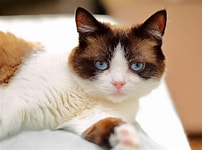
\includegraphics[width=0.85\textwidth]{files/imgs/cat}
	\caption{Cat}
	\label{cat3}
\end{figure}

\begin{table}[H]
	\centering
	\begin{tabular}{|l|l|l|}
		\hline
		Title 1   & Title 2   & Title 3   \\ \hline
		No 1      & No 2      & No 3      \\ \hline
		section 1 & section 2 & section 3 \\ \hline
	\end{tabular}
	\caption{Table example}
    \label{table}
\end{table}

Table \ref{table}

